\documentclass[10pt,a4paper]{article}
\usepackage[utf8]{inputenc}
\usepackage[english]{babel}
\usepackage[english]{isodate}
\usepackage[parfill]{parskip}
\usepackage{amsmath}
\usepackage{mathrsfs}
\usepackage{graphicx}

\DeclareMathOperator*{\argmax}{arg\,max}
\DeclareMathOperator*{\argmin}{arg\,min}



\newenvironment{arglist}
    {\begin{center}
    \begin{tabular}{l|p{12cm}}
    argument & description\\
    \hline
    }
    { 
    \end{tabular} 
    \end{center}
    }


\newenvironment{optarglist}
    {\begin{center}
    \begin{tabular}{l|p{10cm}|l}
    argument & description & default\\
    \hline
    }
    { 
    \end{tabular} 
    \end{center}
    }
\begin{document}
{\bf\huge Figure 2}

All figures use $\varepsilon_0 = 0.2,\mu_0 = 0.15$
Wave profile on $y$-axis with respect to distance on $x$-axis. Left column for $\frac{P_0}{\varepsilon_0} = 0.05, \beta = 0.015$ and right column for $\frac{P_0}{\varepsilon_0} = 0.025, \beta = 0.025$.

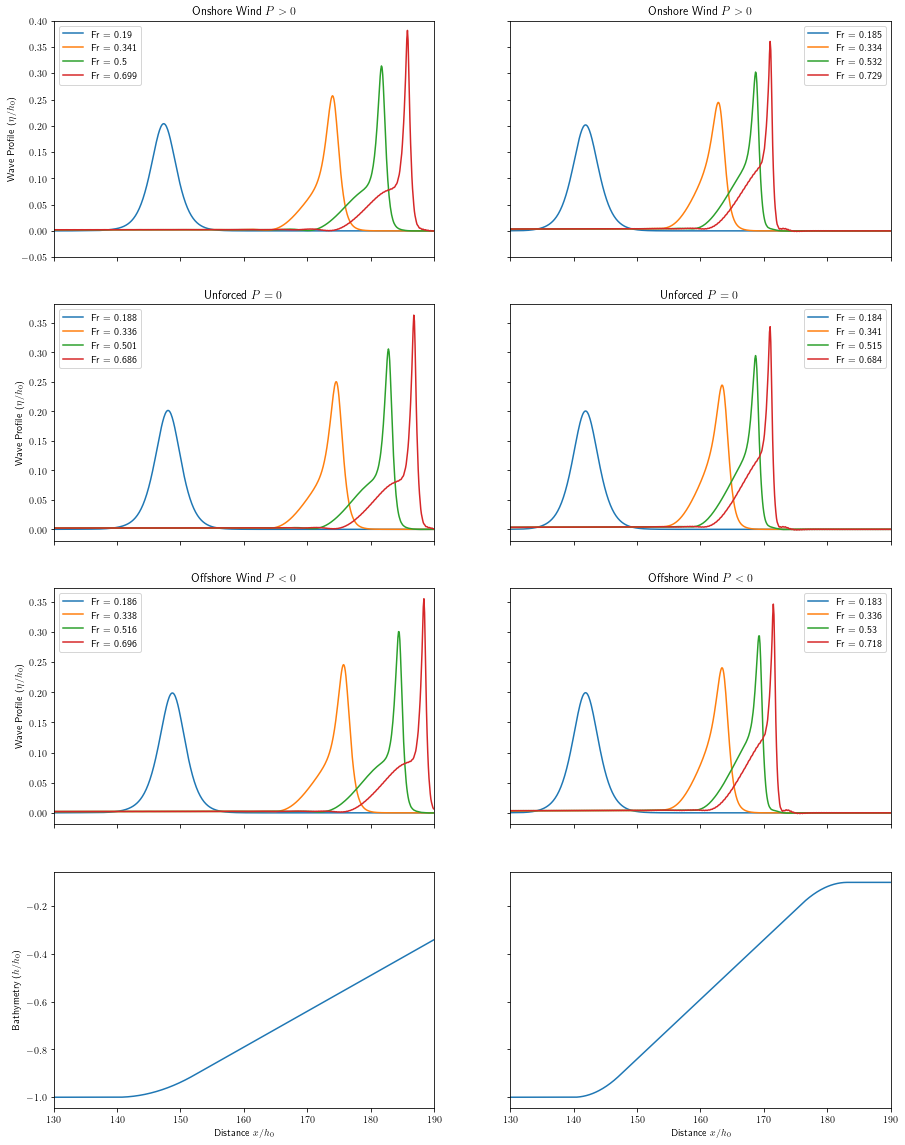
\includegraphics[scale=0.35]{Fig2.png}

Removed the plots at time $0$, and included plots at the thresholds for Fr $=\frac{1}{2}$ and Fr $=\frac{2}{3}$ (By threshold, we mean the first recorded instance of the wave being greater).
The other two are the same as in the manuscript (1/3 threshold, and half the time to that threshold).
\pagebreak


{\bf\huge Figure 3}


We use $\frac{P_0}{\varepsilon_0} = \pm0.05, \beta = 0.015$. Column 1 is positive $P$, column 2 is negative $P$. Row 1 is profile $\eta/h_0$, row2 is slope $\frac{\partial \eta}{\partial x}$, row 3 is velocity $u/\sqrt{gh_0}$.

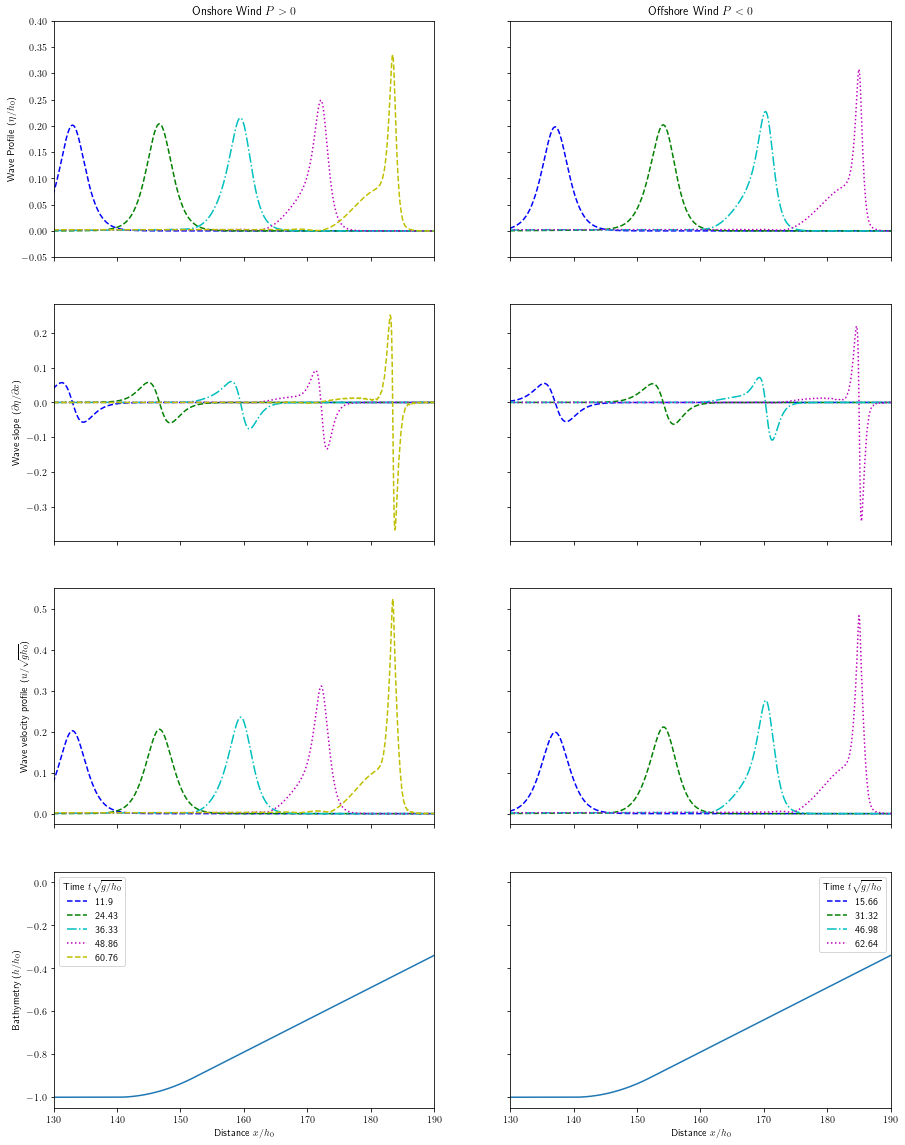
\includegraphics[scale=0.35]{Fig3.png}

We use the same times as the manuscript, except we extend into the future by the same intervals. We should also be careful of $t=0$, because, like in Figure 2, we do not have a time where the wind is ``turned on." Perhaps we should consider re-plotting figures 2 and 3, but with offset times.

Wave velocity is calculated in the same manner as Simulator1D (in fact, we create a new instance of it and use the same functions):
$$|u| = \sqrt{(\phi^S_x)^2 + (1+\eta_x^2)w^2}$$
\pagebreak


{\bf\huge Figure 4}

These are for $\beta = 0.015$.

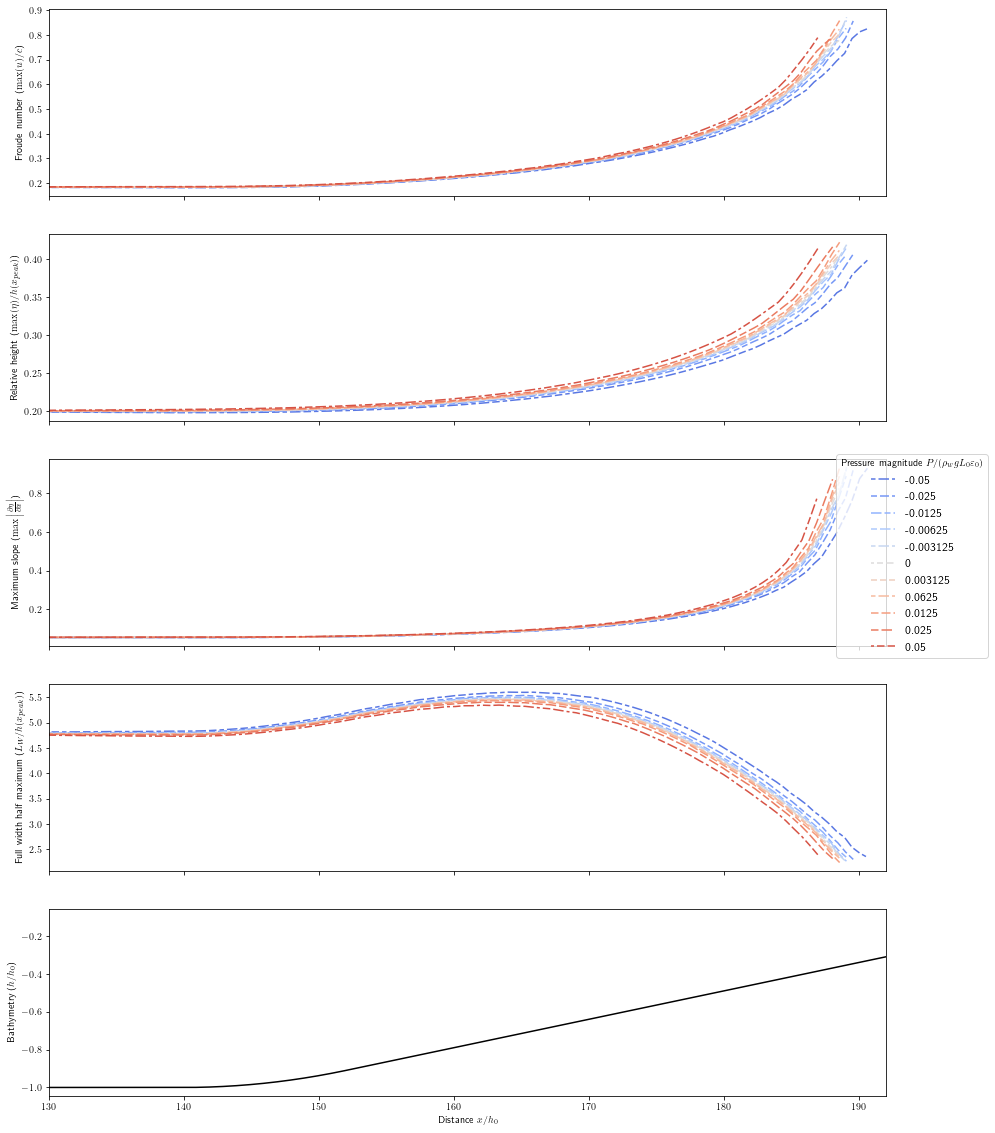
\includegraphics[scale=0.35]{Fig4.png}

We exclude the 0.3 max-Froude number indicator here.
\pagebreak


{\bf\huge Figure 5}

$\Delta x_{pz} = x_{pz} - x_{pz}|_{P=0}$. $x_{pz}$ refers to the $x$ position where the pre-breaking condition Fr $=\frac{1}{3}$ is met relative to the shore ("$x_{shore}$ as the location where the bathymetry would intersect $z=0$ if it had a constant slope $\beta$ without the shallow plateau." (ZF2021, 2.8))
\bigskip

We also examine other breaking conditions.

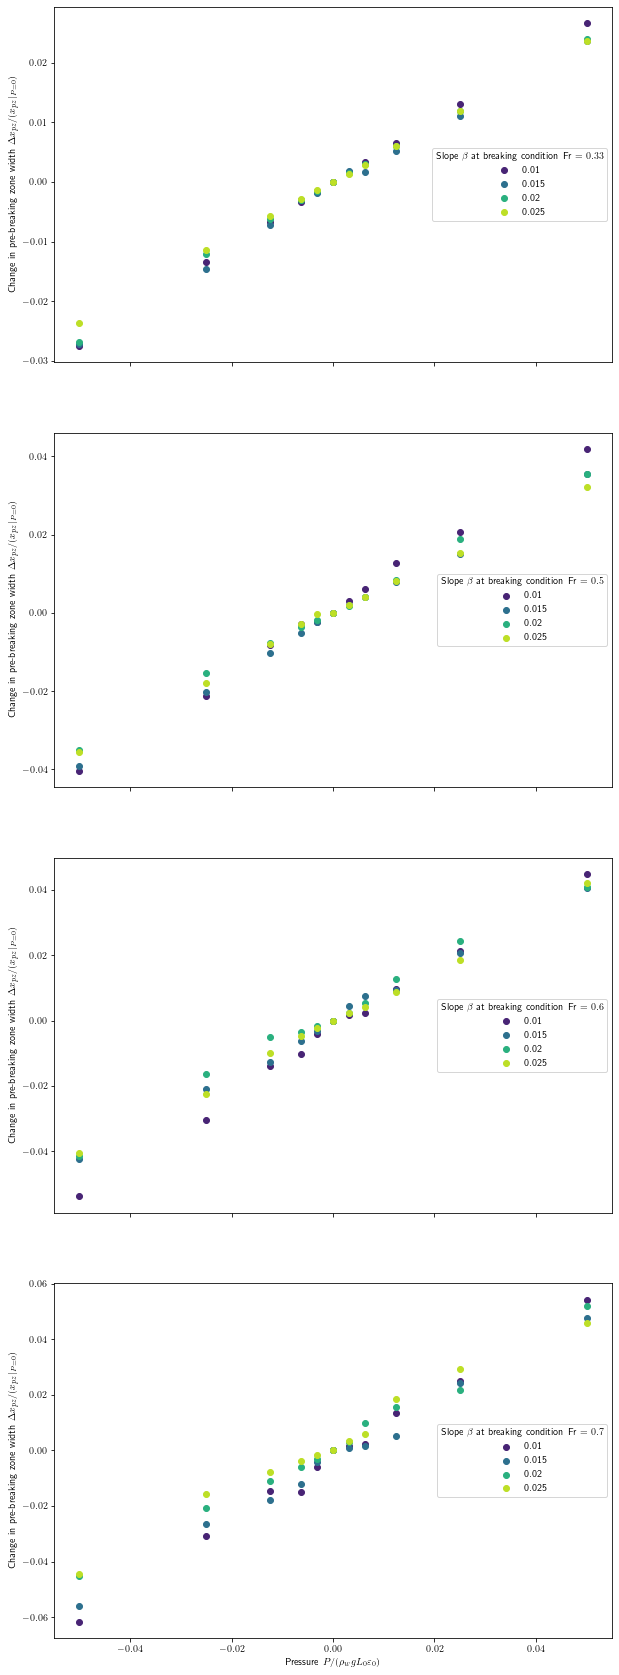
\includegraphics[scale=0.35]{Fig5.png}
\pagebreak


{\bf\huge Figure 6}

Profiles are normalized based by $\max(\eta)$ and offset so that 0 represents $x_{pb}$. Profiles occur at the pre-breaking condition
First row is based on different pressures at $\beta = 0.015$. Second and third are based on different slopes at pressure magnitude $\frac{|P|}{\rho_w g L_0\varepsilon_0} = 0.05$.

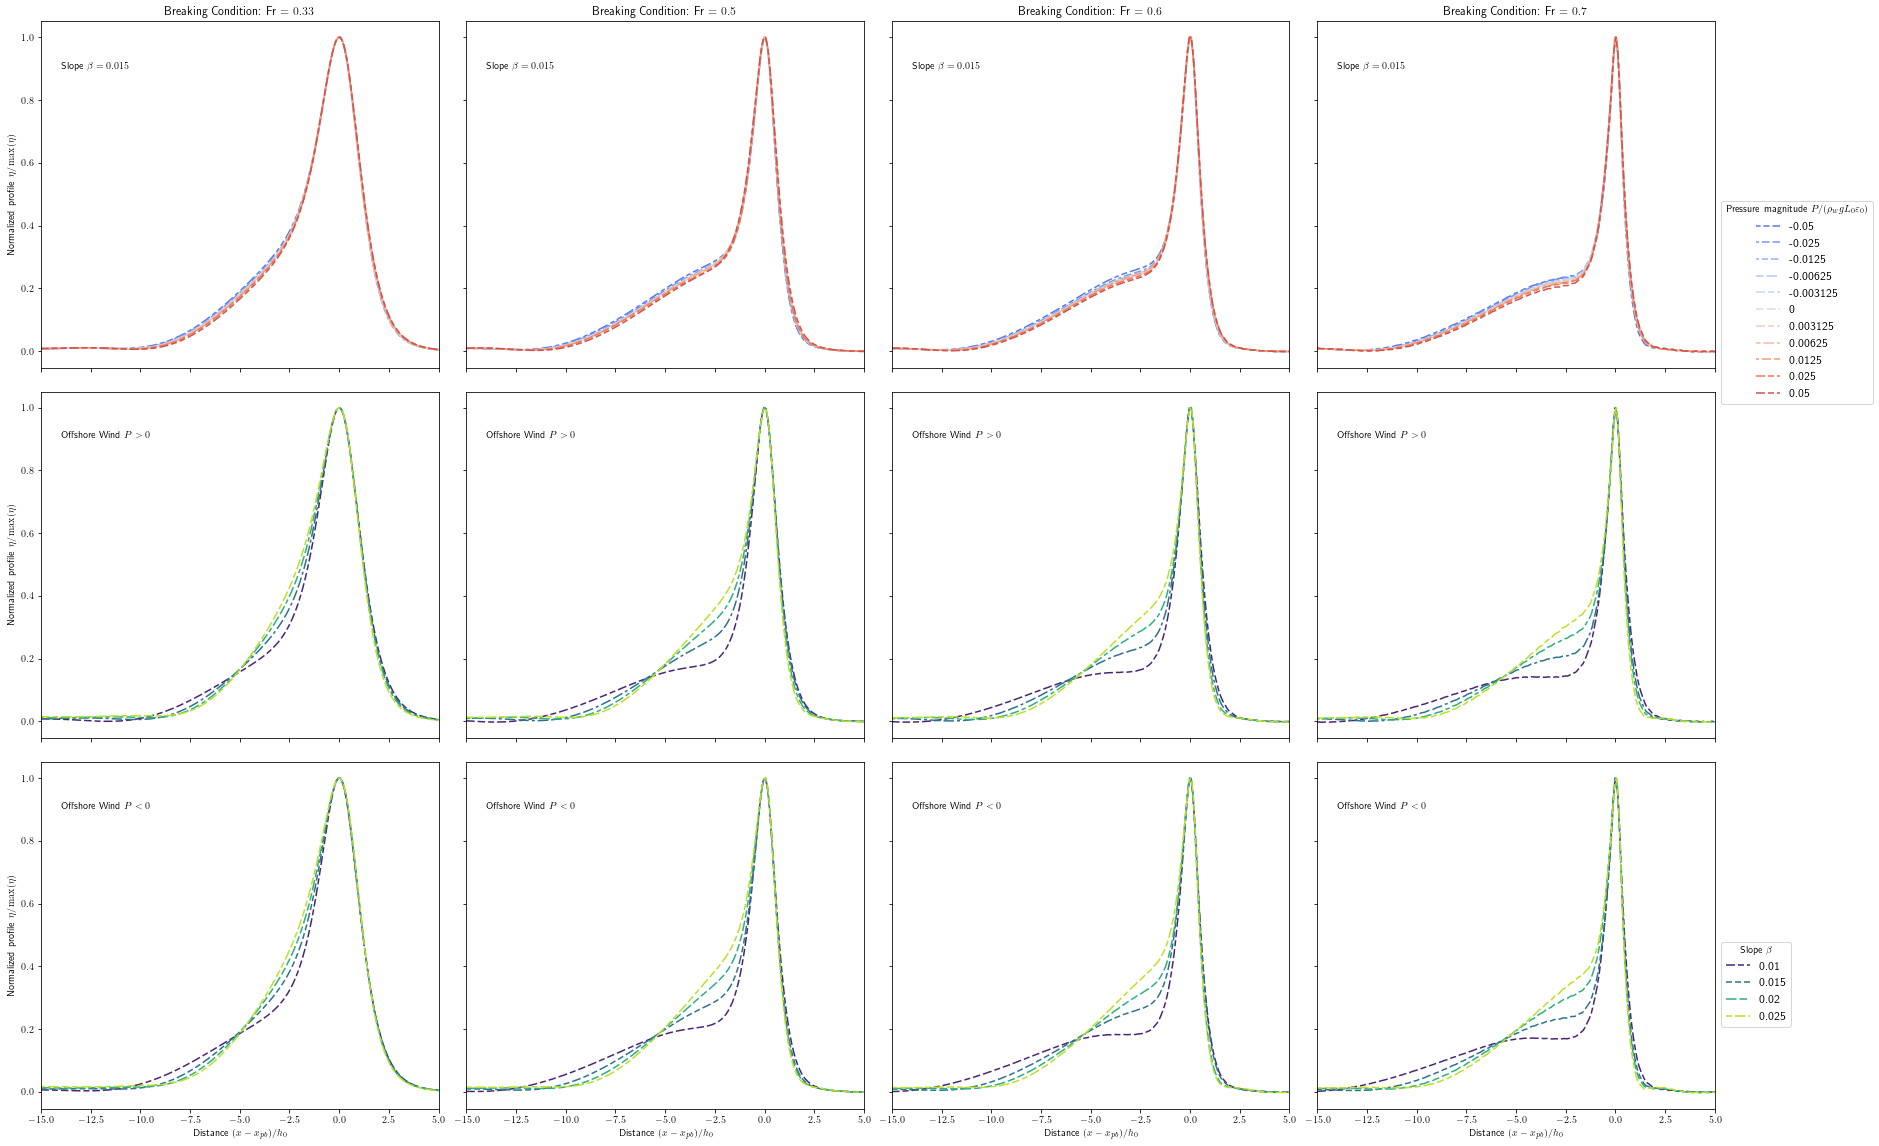
\includegraphics[scale=0.2]{Fig6.png}

We use the same additional breaking conditions as in Figure 5.
\pagebreak


{\bf\huge Figure 7}

We take the same data in figure 5, but plot it with respect to $U/\sqrt{gh(x_{pb})}$. The manuscript takes after Donelan et al. (2006) in approximating
$$\frac{U}{\sqrt{gh}} = 1 \pm \sqrt{\frac15 \left|\frac{P}{\rho_wgL\varepsilon}\right|\frac{4\rho_w}{4.91\sqrt{3\varepsilon} \rho_a}}$$

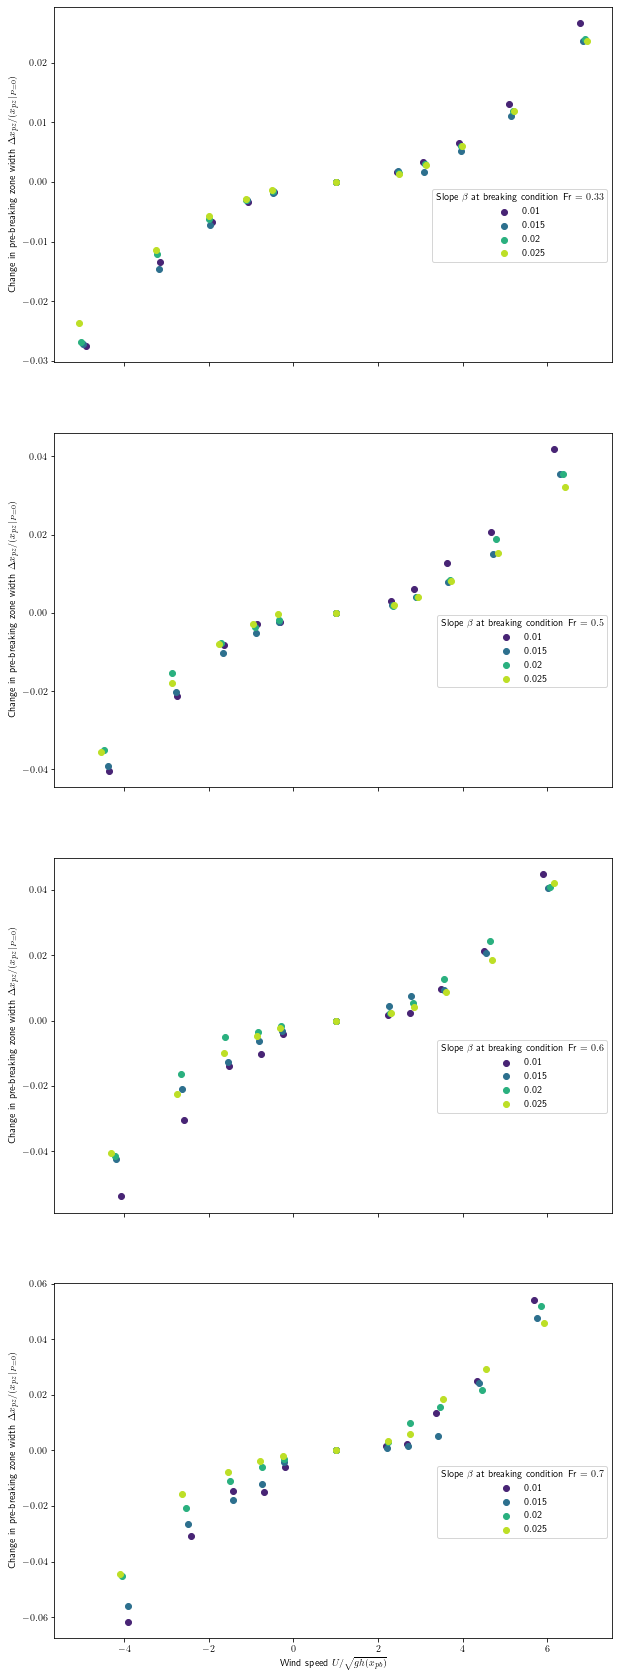
\includegraphics[scale=0.35]{Fig7.png}



\end{document}